\section{Prezentacja warstwy użytkowej projektu}
\subsection{Interfejs użytkownika}
System oferuje dwa główne interfejsy:
\begin{itemize}
\item Interfejs klienta - do składania zamówień
\item Panel administratora - do zarządzania systemem
\end{itemize}

\begin{figure}[H]
\centering
\begin{subfigure}{0.45\textwidth}
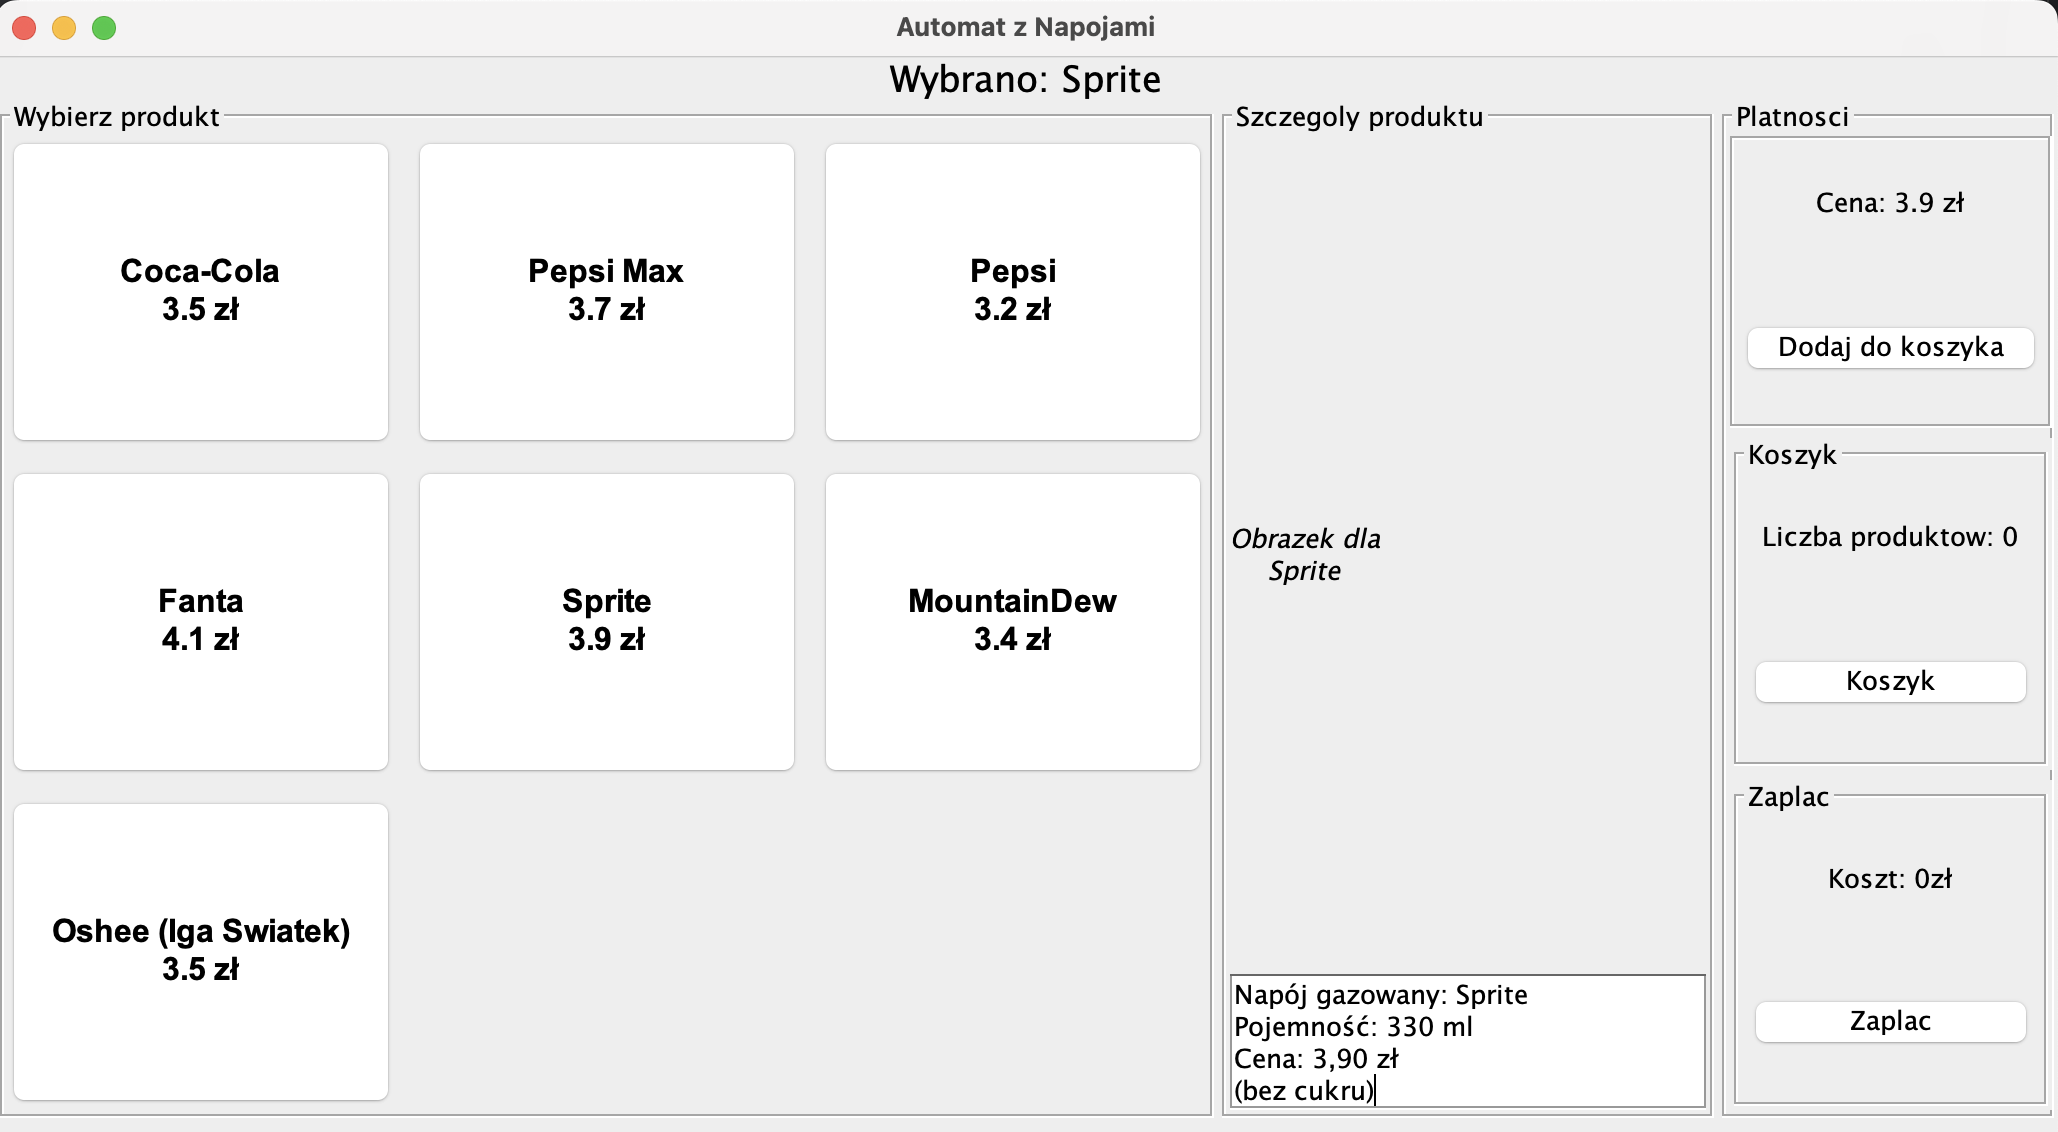
\includegraphics[width=\textwidth]{figures/main_screen.png}
\caption{Ekran główny - wybór produktów}
\label{fig:main_screen}
\end{subfigure}
\begin{subfigure}{0.45\textwidth}
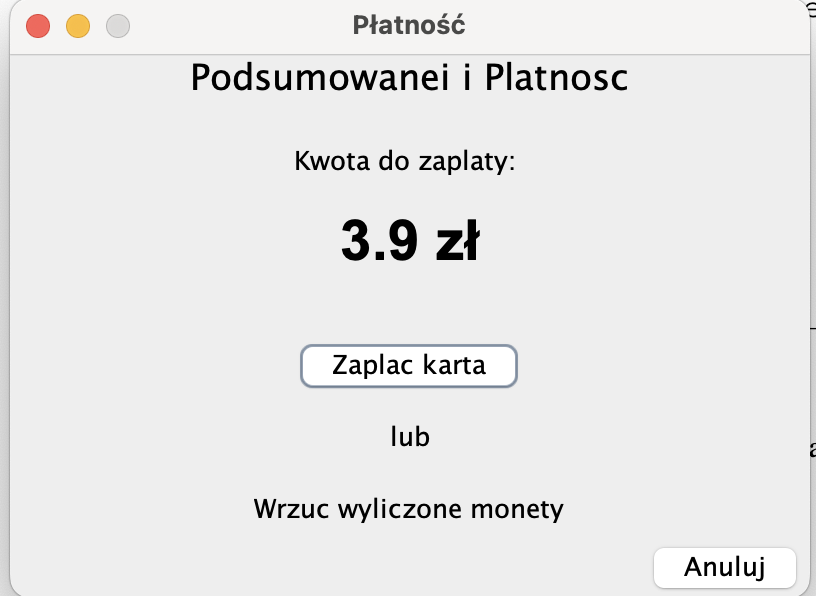
\includegraphics[width=\textwidth]{figures/payment_screen.png}
\caption{Ekran płatności}
\label{fig:payment_screen}
\end{subfigure}
\caption{Podstawowe ekrany systemu}
\end{figure}


\subsection{Przepływ użytkownika}
Typowy scenariusz użycia:
\begin{enumerate}
\item Użytkownik przegląda dostępne produkty
\item Wybiera produkty i dodaje je do koszyka
\item Przechodzi do podsumowania zamówienia
\item Wybiera metodę płatności (gotówka/karta)
\item Otrzymuje potwierdzenie transakcji
\end{enumerate}

\subsection{Panel administratora}
\begin{figure}[H]
\centering
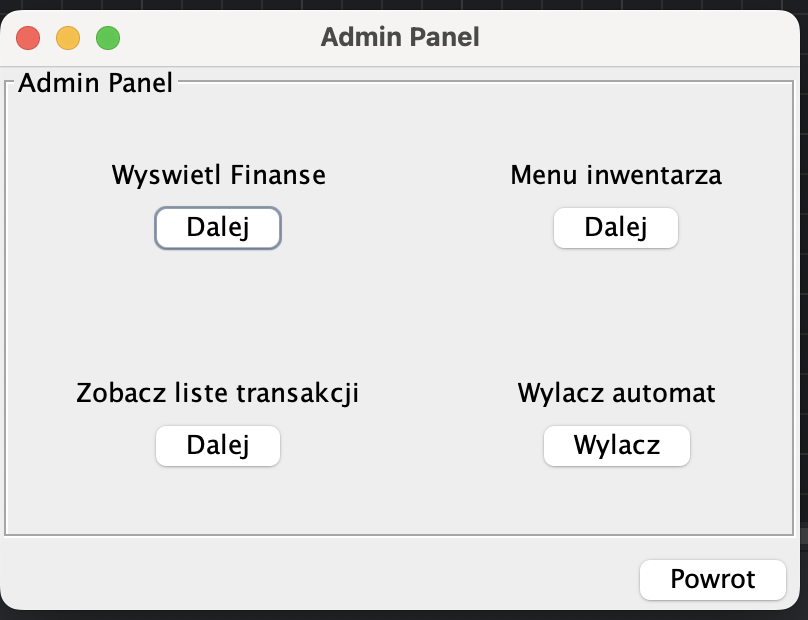
\includegraphics[width=0.7\textwidth]{figures/admin_panel.png}
\caption{Panel administracyjny systemu}
\label{fig:admin_panel}
\end{figure}

Funkcjonalności panelu admina:
\begin{itemize}
\item Zarządzanie produktami (dodawanie, edycja, usuwanie)
\item Przegląd historii transakcji
\item Generowanie raportów finansowych
\item Zarządzanie stanem magazynowym
\end{itemize}